\documentclass[USenglish]{article} 

%% \usepackage{titling}
\usepackage[utf8]{inputenc}           
\usepackage{hyperref}
%%\usepackage[T1]{fontenc,url}
%% \urlstyle{sf}
\usepackage{babel,textcomp,csquotes,graphicx,color}
\usepackage[usenames,dvipsnames]{xcolor}
%%\usepackage[latin1]{inputenc}
\usepackage{eso-pic}
\usepackage{mdframed}
%%\pgfplotsset{compat=1.9}
%% \usepackage[latin1]{inputenc}
\newcommand*{\IconColor}{black}%
\newcommand*{\TrashIcon}{
\includegraphics[scale=0.2]{trash.png}}%
\newcommand*{\InlineTrash}[1]{%
\TrashIcon %
\foreach \x in {#1} {%
    $\boldsymbol{\textcolor{\IconColor}{>}}$ \texttt{\textcolor{\IconColor}{\x}}%
}}%


%%  \setlength{\droptitle}{-10em} 
  \title{Grafterizer Tool for Data Cleaning and Transformation: User Guide} 
%%  \subtitle{User Guide}            


\begin{document}
 \maketitle{}
%%\tableofcontents{} 
This tutorial describes core functionality of the Grafterizer data cleaning and transformation tool …




\section{Transformation metadata}
In this section user defines transformation title and gives a short description of how this transformation processes given data. If user wishes to share transformation, it is possible to expose it as public. In this case other platform users will be able to explore and use given transformation.


After describing transformation metadata user may save transformation by clicking “Save” button {
\includegraphics[scale=0.8]{save.png}} in the top right corner. Transformation may be as well saved later at any moment.


\begin{center}
\begin{figure}[!htbp]
\centering
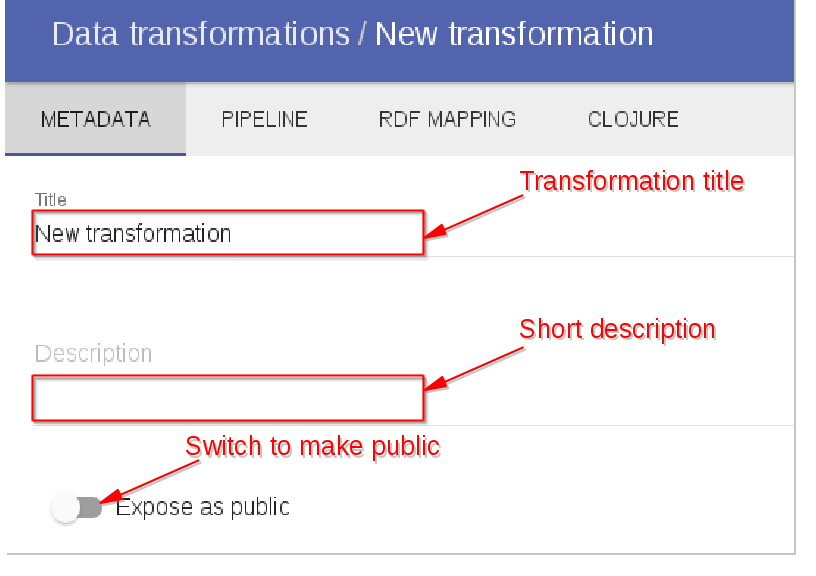
\includegraphics[height=6cm] {meta.png}
 \caption{Transformation metadata \label{meta}}
\end{figure}
\end{center}

\section{Transformation pipeline}
The Grafterizer tool performs tabular data cleaning and transformation with help of “pipeline” concept.  To begin with, each single transformation step is defined as a pipe – a function that performs simple data conversion. The greatest fact about these functions is that they may be combined together in a such way, that output of one pipe acts as an input for another. This way of composition gives a great flexibility and allows to perform rather complex data conversions.

Each transformation starts from reading a dataset, however user do not need to include this step into the transformation pipeline, since this action is performed automatically for each transformation.

To add a first transformation step click the {
\includegraphics[scale=0.8]{add.png}} button next to the pipeline
\begin{center}
\begin{figure}[!htbp]
\centering

\includegraphics[height=2cm] {addpipefunction.png}
 \caption{Add pipe function \label{meta}}
\end{figure}
\end{center}

Now you can see the list of functions you may use to transform your data. Basically each function supports either functionality of Grafter function or combination of several functions to perform a single logical operation(like "Split column").
\begin{center}
\begin{figure}[!htbp]
\centering
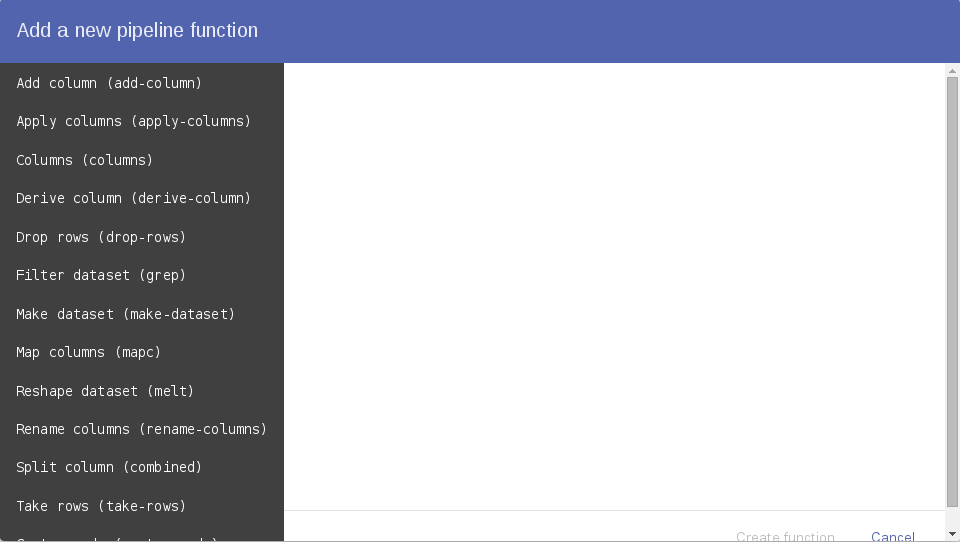
\includegraphics[height=4cm] {functionlist.png}
 \caption{List of available functions \label{meta}}
\end{figure}
\end{center}

 For each option you can see the function description with simple illustrated example by clicking "show/hide documentation" button. You may also leave a note about function you are creating in the "Comment" field. This information helps you and other users of your transformation to understand operations that are performed by this particular function. If you ignore this field, the note will be created automatically based on function parameters you have specified.
 
 \begin{center}
\begin{figure}[!htbp]
\centering
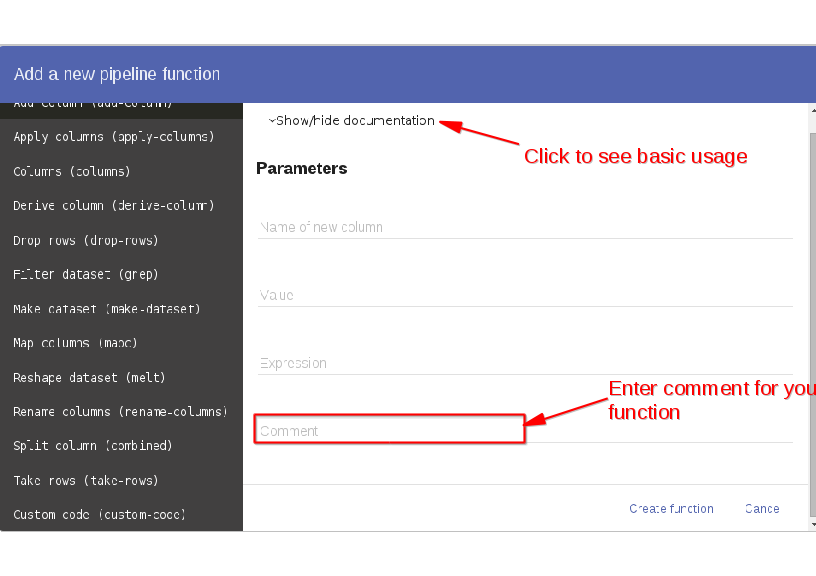
\includegraphics[height=7cm] {pipefunccommon.png}
 \caption{Common operations for all pipe functions \label{meta}}
\end{figure}
\end{center}

  The sections \ref{addcolumn}-\ref{customfunction} provide you with detailed guidelines for each function usage.


\subsection{Add Column \label{addcolumn}}
%% TODO: add add-columns function here
The "Add column" function results in adding a new column to a dataset. To add a new column you should specify column name(this one will be converted to a Clojure keyword automatically) and a value for a new column. This value will be copied into every row within dataset. You allowed as well to use a Clojure expression to obtain value for a new column(this may be useful for instance to obtain current date, time or dataset name). Note that the "Expression" field is prioritized, in other words if you define both value and expression, only expression will be used to get a value for a new column.
 \begin{center}
\begin{figure}[!htbp]
\centering
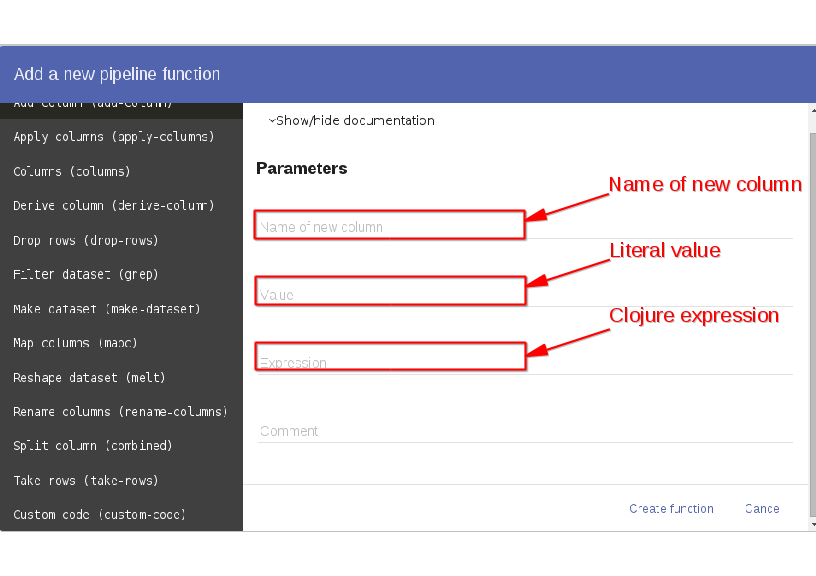
\includegraphics[height=6cm] {addcolumnf.png}
 \caption{Add column function \label{meta}}
\end{figure}
\end{center}

\subsection{Apply Columns}
%% TODO: merge it with mapc??
\subsection{Columns}
%% TODO: add option drop column from dataset
The "Columns" function narrows given dataset to just the specified columns. You may define these columns explicitly by writing their names in "Specify column names" field or by assigning  number of columns to fetch. In second case, dataset will be narrowed to n columns with their names assigned as alphabletical sequence("A","B","C" etc.). If more than 26 columns are fetched column names will count "AA", "AB", "AC" ... "BA", "BB", "BC" etc.

 \begin{center}
\begin{figure}[!htbp]
\centering
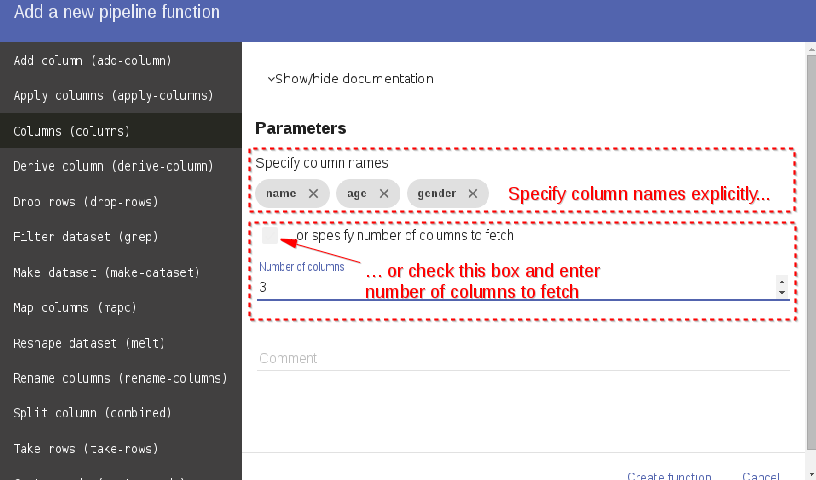
\includegraphics[height=5cm] {columns.png}
 \caption{Columns function \label{meta}}
\end{figure}
\end{center}

\subsection{Derive Column}
%%TODO: describe parameter sending to functions
This function creates a new column in a dataset by applying some transformation to existing column(or columns). To use this function you should specify name for a new column, define one or several columns you are going to use to obtain new value and specify a function you apply to them. This function can be chosen from a drop-down list, which contains some standard functions and custom utility functions. You may define custom utility functions by yourself using Clojure code(see \ref{customFunc}) or use utility functions written by other users.
\begin{mdframed}[hidealllines=true,backgroundcolor=gray!15]
One powerful feature of derive-column and similar pipeline functions is possibility to combine functions you apply to columns in the same way you combine functions in pipelines. Essentially, these are pipelines inside your dataset manipulation pipeline. To add one more "internal" function into your pipeline function, click {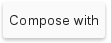
\includegraphics[scale=0.5]{compose.png}} button. Note, that function order is significant in this case. Functions are composed as they appear from top to down. To remove function from composition pipeline click trash icon {
\includegraphics[scale=0.8]{trash.png}} next to the function you wish to delete.
\end{mdframed}

\subsection{Drop Rows}
This function just removes first n rows from a given dataset.
\subsection{Filter Dataset}
This method filters rows in the dataset for matches. This is a rather flexible filtering tool that allows you to filter your data in several different ways.

First field in in "Filter Dataset" parameter list specifies whether filter will be applied to specific column(s) or to all columns in dataset. For latter option just leave this field empty and matching will be performed for each column.

To perform actual data filtering you have several options.

First, it is possible to select only rows containing specified text. For this you enter the text in field marked as "Text to match". %%By default this text is treated as case-sensitive. To perform a case insensitive filtering check the box "ignore case" next to the text field.

You may as well filter dataset with help of regular expressions. By pressing {
\includegraphics[scale=0.6]{tutorial.png}} button next to the "Regular expression" field  you will get short quick start tutorial for pattern usage.

Finally, you may filter dataset by applying utility functions to columns. Note, that the result of function(or combination of functions) will be treated a true/false expression.

The priority of listed option is defined as they appear - from top to down: if "Text to match" field is specified, other fields are ignored, if "Text to match" is ignored, but "Regular expression" is defined -- this one will be used to filter your dataset ignoring functions below(if specified any).
\subsection{Make Dataset}
As its name suggests "Make dataset" operation creates new dataset from its input. If you leave all parameter fields blank new dataset will be created from all the input columns with column names given as simple alphabetic sequence. By checking "move first row to header" option you get all the column names from the first row. First row will be removed from your dataset. You may as well specify column names you wish to take to dataset being created or fetch first n columns.
\subsection{Map Columns}
This method allows you to apply function transformation to column and put the transformed value back to the same column. Transformation is done cell by cell. In parameter list you must specify a column you wish to change and a function that will be used to perform a transformation. You may add as many column-function pairs as you need. 
%%TODO: EITHER describe what's the difference between mapc and apply-columns OR merge these functions into one in tool
\subsection{Reshape Dataset}
Reshape dataset "melts" given dataset in a such way, that each row of new dataset represents a unique combination of variables and values for given column array.
\subsection{Rename Columns}
This operation allows you to rename columns in dataset. To get new names for columns you may either apply function(or function pipeline) to current column names or assign mapping from old to new column names directly.
\subsection{Split Column}
\subsection{Take Rows}
This operation allows you to narrow dataset just to first n rows.
%% TODO: merge with rows(and maybe with drop-rows)
\subsection{Adding Custom Function to Your Pipeline \label{customfunction}}

Some complex transformations cannot be done with help of operations described above. In this case you may need to define your own pipeline functions. This can be done with help of "Custom code" option using Clojure language
\subsection{Creating and editing custom utility functions \label{customFunc}}
%% TODO: 1-add and describe simplified gui for "string transformation" utility functions creation 2- when supported -- describe utility functions sharing
\subsection{Creating and editing prefixers \label{customFunc}}

You may create and edit prefixers in the "Edit prefixers" window. To see this press {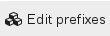
\includegraphics[scale=0.5]{editprefixers.png}} button in the pipeline view. Here you can see the list of all prefixers you created for current transformation. You may add a new prefixer by specifying its name and URI and pressing {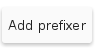
\includegraphics[scale=0.5]{addprefixer.png}} buttom. Created prefixer will instantly appear in the list of prefixers above. It is possible as well to create prefixer by adding some string to the existing one. In this case select a prefixer you wish to choose as base one, enter new prefixer name and string value and press  {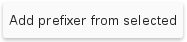
\includegraphics[scale=0.5]{addprefixerfrom.png}}.Now, if the base prefixer is changed, changes will be as well applied to the child prefixers. To remove prefixers select all prefixers you wish to remove and press  {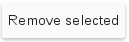
\includegraphics[scale=0.5]{removeprefixers.png}}.


\begin{mdframed}[hidealllines=true,backgroundcolor=gray!10]
\textbf{Example 1.}
The following example illustrates ...
\end{mdframed}




\end{document}